\documentclass[letterpaper, 12 pt]{article}

\setcounter{secnumdepth}{0}
\usepackage{amsmath, amsfonts}
\usepackage{amssymb}
\usepackage{amsthm}
\usepackage{array}
\usepackage{bm}
\usepackage{color}
\usepackage{epsfig}   % for postscript graphics files
\usepackage{fancyhdr}
\usepackage{graphics}
\usepackage{graphicx}
\usepackage{hyperref}
\usepackage{ifthen}
\usepackage{longtable}
\usepackage[margin=2cm,pdftex]{geometry}
\usepackage{mathtools}
\usepackage{multicol}
\usepackage{psfrag}
\usepackage[shortlabels]{enumitem}
\usepackage{subcaption}
\usepackage{tikz}
\usepackage{times}
\usepackage[table]{xcolor}
\usetikzlibrary{arrows.meta}
\DeclarePairedDelimiter{\ceil}{\lceil}{\rceil}

\setlength{\textwidth}{6.5in}
\setlength{\oddsidemargin}{-0.1in}
\setlength{\evensidemargin}{-0.1in}
\setlength{\headheight}{0.1in}
\setlength{\headsep}{0.2in}        %{15pt=0.207555in}
\setlength{\footskip}{0.2in}         %{30pt=0.41511in}
\setlength{\textheight}{9.0in}
\setlength{\hoffset}{0in}
\setlength{\voffset}{0pt}
\setlength{\topmargin}{-0.5in}
\setlength{\parskip}{5pt plus5pt minus5pt}
\setlength{\parindent}{0in}
\renewcommand{\baselinestretch}{1.25}
\usepackage{titling}
\newtheorem{definition}{Definition}
\newcommand{\ds}{\displaystyle}
\newcommand{\p}{\partial}
\newcommand{\R}{\text{I\!R}}
\newcommand{\HRule}{\rule{\linewidth}{0.5mm}}
\newcommand{\Language}{\mathrm{Language}}

\fancyhead{}
\fancyhead[R]{CWID: 103-99-961}
\fancyhead[L]{Homework 4}
\fancyhead[C]{Hayden Pott}
\renewcommand\headrulewidth{0pt}
\fancyfoot{}
\fancyfoot[C]{\thepage}

\pagestyle{fancy}

\begin{document}

\begin{center}
    \Large CSC 310 \\
    Homework 4     \\
    \normalsize
    21 May 2024    \\

    Some work with Landen Nguyen
\end{center}

\section{Lecture 15}

\begin{enumerate}
    \item \char`[True or False] The intersection of
        $L_1=\text{Language}(\bm{a^*b^*})$ and $L_2=\Language(a^Nb^N: N \geq
        0)$ is a Context Free Language.

    \item \char`[True or False] The complement of $L$ (i.e., $L'$) is Context Free, when $L$ is
        defined as all words over the alphabet $\{a, b\}$ where the total number
        of a's and b's are unequal.

    \item \char`[True or False] Since Equivalence is undecidable for Context
        Free Languages it is never possible to tell whether two given CFGs
        define the same language.

    \item Using the algorithm of Theorem 36, prove that the union of $L_1 =
        \Language(a^Nb^{2N}: N \geq 0)$ and $L_2 = \Language(a^Nb^Ma^{N+M} : N
        \geq 0, M \geq 0)$ is Context Free

    \item Using the algorithm of Th. 38 prove that $\bm{L^*}$ is Context Free,
        where $L = Language(a^Nb^{2N}: N \geq 0)$.

    \item Give an example of two Context Free Languages where the intersection
        of those two languages is, itself, Context Free.

\end{enumerate}

\section{Lecture 16}

\begin{enumerate}

    \item Using the TM of Slide 17, trace the successful path of input string
        ``aabbaa''.

    \item Using the TM of Slide 17, trace the unsuccessful path of the input
        string ``aabaaa''.

    \item Construct a TM for the language $a^N b a^N: N \geq 1$

    \item Using the TM of the previous problem, trace the successful path of the
        input string ``aabaa''.

    \item Using the same TM, trace the unsuccessful path of the input string ``abaa''.

\end{enumerate}

\section{Lecture 17}

\begin{enumerate}

    \item Using the PM of Slide 6, trace the unsuccessful path of input string
        ``aabbbaa''.

    \item Construct a PM for the language $a^Nba^N: N \geq 0$

    \item Using the 2PDA for $a^Nb^Na^N: N \geq 1$ of Slide 8, trace the
        successful path of input string ``aaabbbaaa''. For your trace construct
        a table showing (a) the State, (b) the input tape, bolding the character
        being read, (c) the contents of Stack $\alpha$, and (d) the contents of
        Stack $\beta$. See page 481 of your text for an example. \\
        \textbf{ANS:} \\
        \begin{center}
          \rowcolors{2}{gray!25}{white}
            \begin{tabular}{| c c c c |}
                \rowcolor{gray!50}
                State             & Input Tape                            & $\alpha$                    & $\beta$ \\
                Start         & $aaabbbaaa                   \Delta $ & $\Delta$                    & $\Delta$ \\
                Read$_1$      & $\underline{a}aabbbaaa       \Delta $ & $\Delta$                    & $\Delta$ \\
                Push$_\alpha$ & $aaabbbaaa                   \Delta $ & $a \Delta$                  & $\Delta$ \\
                Read$_1$      & $a\underline{a}abbbaaa       \Delta $ & $a \Delta$                  & $\Delta$ \\
                Push$_\alpha$ & $aaabbbaaa                   \Delta $ & $a a \Delta$                & $\Delta$ \\
                Read$_1$      & $aa\underline{a}bbbaaa       \Delta $ & $a a \Delta$                & $\Delta$ \\
                Push$_\alpha$ & $aaabbbaaa                   \Delta $ & $a a a \Delta$              & $\Delta$ \\
                Read$_1$      & $aaa\underline{b}bbaaa       \Delta $ & $a a a \Delta$              & $\Delta$ \\
                Pop$_\alpha$  & $aaabbbaaa                   \Delta $ & $\underline{a} a a \Delta$  & $\Delta$ \\
                Push$_\beta$  & $aaabbbaaa                   \Delta $ & $a a \Delta$                & $b \Delta$ \\
                Read$_2$      & $aaab\underline{b}baaa       \Delta $ & $a a \Delta$                & $b \Delta$ \\
                Pop$_\alpha$  & $aaabbbaaa                   \Delta $ & $\underline{a} a \Delta$    & $b \Delta$ \\
                Push$_\beta$  & $aaabbbaaa                   \Delta $ & $a \Delta$                  & $b b \Delta$ \\
                Read$_2$      & $aaabb\underline{b}aaa       \Delta $ & $a \Delta$                  & $b b \Delta$ \\
                Pop$_\alpha$  & $aaabbbaaa                   \Delta $ & $\underline{a} \Delta$      & $b b \Delta$ \\
                Push$_\beta$  & $aaabbbaaa                   \Delta $ & $\Delta$                    & $b b b \Delta$ \\
                Read$_2$      & $aaabbb\underline{a}aa       \Delta $ & $\Delta$                    & $b b b \Delta$ \\
                Pop$_\alpha$  & $aaabbbaaa                   \Delta $ & $\underline{\Delta} \Delta$ & $b b b \Delta$ \\
                Pop$_\beta$   & $aaabbbaaa                   \Delta $ & $\Delta$                    & $\underline{b} b b \Delta$ \\
                Read$_3$      & $aaabbba\underline{a}a       \Delta $ & $\Delta$                    & $b b \Delta$ \\
                Pop$_\beta$   & $aaabbbaaa                   \Delta $ & $\Delta$                    & $\underline{b} b \Delta$ \\
                Read$_3$      & $aaabbbaa\underline{a}       \Delta $ & $\Delta$                    & $b \Delta$ \\
                Pop$_\beta$   & $aaabbbaaa                   \Delta $ & $\Delta$                    & $\underline{b} \Delta$ \\
                Read$_3$      & $aaabbbaaa \underline{\Delta} $       & $\Delta$                    & $\Delta$ \\
                Pop$_\beta$   & $aaabbbaaa                   \Delta $ & $\Delta$                    & $\underline{\Delta} \Delta$ \\
                Accept        & $aaabbbaaa                   \Delta $ & $\Delta$                    & $\Delta$ \\
            \end{tabular}
        \end{center}

    \item Construct a 2PDA for $a^Nb^Na^Nb^N: N \geq 1$ (Use the 2PDA of Slide 8 as a guide).

    \item What language is defined by the following Context Sensitive Grammar?
        \begin{enumerate}[1.]
            \item $S \to abc$
            \item $S \to aAbc$
            \item $Ab \to bA$
            \item $Ac \to Bbcc$
            \item $bB \to Bb$
            \item $aB \to aaA$
            \item $aB \to aa$
        \end{enumerate}

    \item Show the derivation of a word in the language of problem 5, where the
        length of that word is at least six. Use the technique shown at the
        bottom of Slide 21 to visualize your derivation.

\end{enumerate}

\section{Lecture 17}

\begin{enumerate}

    \item \char`[True or False] $\bm{a^*b^*}$ is a recursively Enumerable
        language.

    \item \char`[True or False] $a^Nb^Na^N: N \geq 0$ is a Context Free
        language.

    \item \char`[True or False] Every Recursive language is also Recursively
        Enumerable.

    \item \char`[True or False] Some languages are not Recursively Enumerable.

    \item \char`[True or False] Because membership is not decidable for
        Recursively Enumerable languages, it is never possible to tell whether a
        word W is a member of Recursively Enumerable language L.

    \item Using the CWL of Slide 16 from today’s lecture, encode the Turing
        Machine of Slide 18 of Lecture 16. Note that Node 2 will need to be
        renamed Node 3 to be consistent with our new naming convention.

    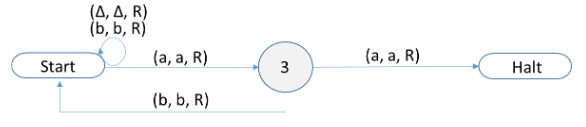
\includegraphics[width=\linewidth]{hw4-q18-6.png}

\end{enumerate}

\end{document}
